% LaTeX template for creating an MNRAS paper
%
% v3.2 released 20 July 2023
% (version numbers match those of mnras.cls)
%
% Copyright (C) Royal Astronomical Society 2015
% Authors:
% Keith T. Smith (Royal Astronomical Society)

%%%%%%%%%%%%%%%%%%%%%%%%%%%%%%%%%%%%%%%%%%%%%%%%%%%%%%%%%%%%%%%%%%%%%%%%%%%%%%%%%%%%%%%%%%%%%%%%%%%%
% Basic setup. Most papers should leave these options alone.
\documentclass[fleqn,usenatbib]{mnras}

% MNRAS is set in Times font. If you don't have this installed (most LaTeX
% installations will be fine) or prefer the old Computer Modern fonts, comment
% out the following line
\usepackage{newtxtext,newtxmath}
% Depending on your LaTeX fonts installation, you might get better results with one of these:
%\usepackage{mathptmx}
%\usepackage{txfonts}

% Use vector fonts, so it zooms properly in on-screen viewing software
% Don't change these lines unless you know what you are doing
\usepackage[T1]{fontenc}

% Allow "Thomas van Noord" and "Simon de Laguarde" and alike to be sorted by "N" and "L" etc. in the bibliography.
% Write the name in the bibliography as "\VAN{Noord}{Van}{van} Noord, Thomas"
\DeclareRobustCommand{\VAN}[3]{#2}
\let\VANthebibliography\thebibliography
\def\thebibliography{\DeclareRobustCommand{\VAN}[3]{##3}\VANthebibliography}


%%%%% AUTHORS - PLACE YOUR OWN PACKAGES HERE %%%%%

% Only include extra packages if you really need them. Avoid using amssymb if newtxmath is enabled, as these packages can cause conflicts. newtxmatch covers the same math symbols while producing a consistent Times New Roman font. Common packages are:
\usepackage{graphicx}	
\usepackage{amsmath}	
\usepackage{physics}
\usepackage{enumitem}
\usepackage{anyfontsize}
\usepackage{placeins}
\usepackage{cleveref}


%%%%%%%%%%%%%%%%%%%%%%%%%%%%%%%%%%%%%%%%%%%%%%%%%%%%%%%%%%%%%%%%%%%%%%%%%%%%%%%%%%%%%%%%%%%%%%%%%%%%

%%%%% AUTHORS - PLACE YOUR OWN COMMANDS HERE %%%%%

% Please keep new commands to a minimum, and use \newcommand not \def to avoid
% overwriting existing commands. Example:
%\newcommand{\pcm}{\,cm$^{-2}$}	% per cm-squared

\graphicspath{{images/}}
%\raggedbottom               %This will let the height of the textblock vary from page to page. 

% Command to use placeins with \subsection
\makeatletter
\AtBeginDocument{%
  \expandafter\renewcommand\expandafter\subsection\expandafter
    {\expandafter\@fb@secFB\subsection}%
  \newcommand\@fb@secFB{\FloatBarrier
    \gdef\@fb@afterHHook{\@fb@topbarrier \gdef\@fb@afterHHook{}}}%
  \g@addto@macro\@afterheading{\@fb@afterHHook}%
  \gdef\@fb@afterHHook{}%
}
\makeatother

%%%%%%%%%%%%%%%%%%%%%%%%%%%%%%%%%%%%%%%%%%%%%%%%%%%%%%%%%%%%%%%%%%%%%%%%%%%%%%%%%%%%%%%%%%%%%%%%%%%%


%%%%%%%%%%%%%%%%%%% TITLE PAGE %%%%%%%%%%%%%%%%%%%%%%%%%%%%%%%%%%%%%%%%%%%%%%%%%%%%%%%%%%%%%%%%%%%%%

% Title of the paper, and the short title which is used in the headers.
% Keep the title short and informative.
\title[]{Simulating the formation of supermassive black hole binaries}

% The list of authors, and the short list which is used in the headers.
% If you need two or more lines of authors, add an extra line using \newauthor
\author[Marco Bianchi]{
Marco Bianchi
\\
% List of institutions
University of Milano-Bicocca, Physics Department, Astrophysics and Space Physics master degree\\
Dynamics of Stellar Systems 2023-2024
}

% Enter the current year, for the copyright statements etc.
\pubyear{2025}

% Don't change these lines
\begin{document}
\label{firstpage}
\pagerange{\pageref{firstpage}--\pageref{lastpage}}
\maketitle

% Abstract of the paper
\begin{abstract}
  \large The Cocoon Nebula (IC 5146) is an HII region embedded within the Barnard 168 absorption nebula, making it a prime target for studying dust extinction. 
  We obtained photometric images of IC 5146 using H$\alpha$ and H$\beta$ filters and analyzed the Balmer decrement to create a two-dimensional map of the color excess E(B-V), which serves as a proxy for dust column density. 
  Our results indicate a median E(B-V) of $\approx 0.461 \pm 0.008$ across the nebula, with a standard deviation of $\approx 0.34$. 
  A comparison with previous spectroscopic studies reveals a discrepancy in E(B-V) estimates, which we attribute to methodological differences in spatial sampling.\\
  Furthermore, given the nebula's nearly spherical morphology and its ionization by a single B0.5V-type star (BD+46 3474), we tested the Strömgren sphere model. 
  By incorporating literature values for electron density and temperature, as well as for the radius and temperature of BD+46 3474, we derived a Strömgren radius of $\approx 1.14$ pc, which is broadly consistent with the observed nebular size. 
  However, uncertainties in the nebula's distance and simplifying assumptions in the Strömgren model highlight the need for more detailed modeling.
\end{abstract} 
%%%%%%%%%%%%%%%%%%%%%%%%%%%%%%%%%%%%%%%%%%%%%%%%%%%%%%%%%%%%%%%%%%%%%%%%%%%%%%%%%%%%%%%%%%%%%%%%%%%%




%%%%%%%%%%%%%%%%% BODY OF PAPER %%%%%%%%%%%%%%%%%%%%%%%%%%%%%%%%%%%%%%%%%%%%%%%%%%%%%%%%%%%%%%%%%%%%

\section{Introduction}\label{sec:introduction}
It is a well-established fact that most galaxies host a massive black hole (MBH) at their center, with masses ranging from a few million to several billion solar masses. In the latter case, these are referred to as supermassive black holes (SMBHs).
On the other hand, galactic mergers are expected to be frequent events in the Universe, and indeed we observe many galaxies in various stages of the merging process.
This raises the question of what happens to MBHs during these mergers.
The most likely outcome is the formation of a MBH binary at the center of the newly formed galaxy.
The process leading to the formation and the evolution of such a bound state is complex and involves several stages, which were originally outlined by \cite{Begelman1980}.

\subsection{Dynamical friction}\label{sec:introduction_dynamical_friction}
In this work, we focus on the process that causes the MBHs to sink towards the core of the merger remnant, a mechanism known as \textbf{dynamical friction}.
The main idea is that a massive object moving through a stellar system will transfer energy and angular momentum to the surrounding stars, slowing down and thus spiraling inward, toward the center of mass of the system. Although the object may gain speed as it moves into a region with deeper gravitational potential, this does not contradic the previous statement, since the total orbital energy is still decreasing.
The mathematical formalization of dynamical friction was first proposed by \cite{Chandrasekhar1943}, based on the assumption that the stellar background is homogeneous and isotropic.
In particular, the perturber is subject to a deceleration given by the following equation:
{\fontsize{8.5pt}{8.5pt}\begin{equation}
    \dfrac{d\vec{v}_M}{dt} \, = \, -16 \pi^2 G^2 m \left(m+M\right) \ln \Lambda \left[\int^{v_M}_0 f(v_m) v_m^2 dv_m\right] \dfrac{\vec{v}_M}{v_M^3},
    \label{eq:chandrasekhar}
\end{equation}}
where $\ln \Lambda$ is the Coulomb logarithm (which depends on the maximum and minimum impact parameters of the interaction), $m$ is the mass of the background particles, $M$ is the mass of the perturber, and $f(v_m)$ is the distribution function of the background particles.
Dynamical friction is most efficient when $v_M \simeq v_m$, which is typically the case during the inspiral, and becomes negligible for $v_M \ll v_m$ or $v_M \gg v_m$.

Once the MBHs have sunk to the center of the merger remnant and their separation is such that each is primarily influenced by the gravitational pull of the other, they form a bound state.
The critical separation at which this occurs can be approximated by the \textbf{influence radius}, i.e., the distance at which the gravitational potential energy of the MBH is comparable to the kinetic energy of the surrounding stars:
{\fontsize{7.4pt}{7.4pt}\begin{equation}
    r_\text{inf} = \dfrac{GM}{\sigma^2} 
    \approx 1 \left(\dfrac{M}{10^6 M_\odot}\right) \left(\dfrac{\sigma}{70 \text{km/s}}\right)^{-2} \text{pc} 
    \approx 50 \left(\dfrac{M}{10^9 M_\odot}\right) \left(\dfrac{\sigma}{300 \text{km/s}}\right)^{-2} \text{pc} ,
    \label{eq:influence_radius}
\end{equation}}
where $\sigma$ is the velocity dispersion of the stars surrounding the MBH.

The formation of the binary causes a sudden change in the velocities of the MBHs relative to the surrounding stars, making dynamical friction inefficient.
Morever, once the MBHs are bound, dynamical friction acts of the center of mass of the binary, rather than on the individual MBHs.

The next step is to determine whether other mechanisms can reduce the binary separation further, eventually leading to coalescence.
It is well known that compact-object binaries lose energy and angular momentum via gravitational wave emission, thus shrinking their orbits.
However, this process becomes efficient only when the binary separation is already very small, of the order of a few milliparsecs.
We therefore need to identify a mechanism capable of bridging the gap from parsecs to milliparsecs.
This is the so-called \textbf{final-parsec problem}, which has been the subject of extensive research in the past decades.
The most promising solution is \textbf{stellar hardening}, a process in which stars undergo three-body interactions with the binary, extracting energy and angular momentum from it.
More informations on this process can be found in \cite{Quinlan1996}.
%%%%%%%%%%%%%%%%%%%%%%%%%%%%%%%%%%%%%%%%%%%%%%%%%%

\subsection{Modeling galactic bulges with Barnes-Hut treecode}\label{sec:introduction_models}
The efficiency of dynamical friction depends on the density and velocity distribution of the stars that constitute the bulge of the merger remnant.
This is typically modeled as a spherically symmetric distribution of particles, with a density profile that decays with distance from the center.
The model most commonly used in analytical calculations is the \textbf{singular isothermal sphere} (SIS), whose density and mass profiles are given by:
\begin{equation}
    \rho_\text{SIS}(r) = \dfrac{\sigma^2}{2 \pi G r^2} \:\: , \:\: M_\text{SIS}(r) = \dfrac{2 \sigma^2}{G} r \:\:.
    \label{eq:sis_density}
\end{equation}
However, this model is not realistic, as it diverges at $r=0$ and predicts an infinite total mass.
In the next section, we will introduce more physical alternatives that remain spherically symmetric but possess finite total mass.

In any case, modeling a galactic bulge requires a large number of particles, typically of the order of $N \approx 10^6$.
Therefore, the use of direct N-body simulations — which have a computational complexity of $\mathcal{O}(N^2)$ — is not feasible.
Instead, a \textbf{treecode} algorithm allows to approximate the gravitational potential of a system of particles by organizing them into a hierarchical tree structure.
If the size of a cell — as seen from the point where the force is being computed — is sufficiently small, the group can be treated as a single particle, thus reducing the number of pairwise interactions to $\mathcal{O}(N \log N)$.
In particular, we will use the treecode developed by \cite{Barnes1986}, which is a well-known implementation of this algorithm.
It allows the user to set the following parameters:
\begin{itemize}[wide, labelwidth=!, itemindent=!, labelindent=0pt, itemsep=0.1em]
  \item \textbf{Integration time-step $dt$:} the time interval between two consecutive updates of particle positions and velocities. It must be small enough to ensure accurate integration of the system's evolution, but large enough to keep the computational time manageable. 
  \item \textbf{Opening angle $\theta$:} determines the accuracy of the treecode approximation by controlling how small the angle subtended by a cell must be before it can be treated as a single particle.
  \item \textbf{Softening radius $\epsilon$:} gravitational forces are smoothed by replacing each particle with a Plummer sphere of scale length $\epsilon$, preventing the force from diverging at small distances and producing non-physical interactions. 
\end{itemize}
%%%%%%%%%%%%%%%%%%%%%%%%%%%%%%%%%%%%%%%%%%%%%%%%%%
%%%%%%%%%%%%%%%%%%%%%%%%%%%%%%%%%%%%%%%%%%%%%%%%%%%%%%%%%%%%%%%%%%%%%%%%%%%%%%%%%%%%%%%%%%%%%%%%%%%%


\section{Distributing particles according to the isothermal sphere, King, and Hernquist models}\label{sec:observation}
As introduced in the previous section, the SIS density profile of Eq. \ref{eq:sis_density} is not physical, as it diverges at $r=0$ and yields an infinite total mass.
Therefore, a realistic density profile must have a finite central value and decrease faster than $r^{-3}$ at large distances.
In this section, we begin with a naive regularization of the SIS model and then we introduce two more realistic models commonly used to describe the density distribution of galactic bulges.
For each model, we derive the radial probability distribution function (PDF) of the particles, which can be used to sample their positions, and the analogous velocity PDF, which can be used to assign initial velocities.
\vspace{0.5em}

For any spherically symmetric model, the angular PDFs of the particles are given by:
\begin{equation}
    p(\phi) = \dfrac{1}{2 \pi} \:\: \text{and} \:\: p(\theta) = \dfrac{\sin \theta}{2}  \:\: ,
    \label{eq:angular_pdf}
\end{equation}
which can be easily integrated to obtain the cumulative distribution functions (CDFs).
The \textbf{direct Monte Carlo sampling method} enables the sampling of each angle by generating CDF values $P \in [0,1]$ from a uniform distribution and inverting the CDF formula:
\begin{equation}
    \phi(P_\phi) = 2 \pi P_\phi \:\: , \:\: \theta(P_\theta) = \arccos\left(1 - 2 P_\theta\right) \:\: .
    \label{eq:angular_sampling}
\end{equation}

\subsection{Regularized isothermal sphere}\label{sec:isothermal_sphere}
The first model we consider is a regularized version of the SIS, which we refer to as the \textbf{regularized isothermal sphere} (RIS).
The idea is to cure the divergence at $r=0$ by introducing a softening radius $r_\text{soft}$ (not to be confused with the softening radius $\epsilon$ used in the treecode).
We also apply an exponential cutoff at large distances, governed by a scale length $R$.
The resulting density profile is:
\begin{equation}
    \rho_\text{RIS}(r) = \dfrac{\sigma^2}{2 \pi G \left(r + r_\text{soft}\right)^2} e^{-r/R} \:\: .
    \label{eq:ris_density}
\end{equation}
Given the density profile, the radial PDF of the particles is:
\begin{equation}
    p(r)dr = \dfrac{4\pi r^2 \rho(r)}{M_\text{tot}} dr\:\: ,
    \label{eq:radial_pdf}
\end{equation}
which in the case of the RIS model becomes:
\begin{equation}
    p_\text{RIS}(r)dr \propto \dfrac{r^2 e^{-r/R}}{\left(r + r_\text{soft}\right)^2} dr\:\: .
    \label{eq:ris_pdf}
\end{equation}
Integrating $p_\text{RIS}(r)$ to obtain the CDF is not trivial, and inverting it analytically is even more challenging.
However, we can use the \textbf{acceptance-rejection sampling method} to draw samples from this PDF, employing a decreasing exponential function as the proposal distribution.
This procedure, combined with the angular sampling from Eq. \ref{eq:angular_sampling}, allows us to generate particle positions according to the RIS model.
\vspace{0.5em}

To evolve the system, we must assign an initial velocity to each particle.
Ideally, this requires sampling from the conditional velocity PDF at radius $r$, which is given by:
\begin{equation}
    p(v|r)dv = \dfrac{f(E(v|r))}{n(r)} v^2 dv \:\: ,
    \label{eq:velocity_pdf}
\end{equation}
where $n(r)$ is the number density at radius $r$, and $f(E(r,v))$ is the distribution function describing the number of the particles per unit of phase-space volume.
Given $\rho(r)$, one could derive the gravitational potential $\Phi(r)$ via the Poisson equation, and then obtain the distribution function $f(E(r,v))$ by solving the Eddington equation.
However, this is a complex task that lies beyond the scope of this simplified model.
Therefore, we approximate the RIS distribution function using that of the SIS model: a three-dimensional Maxwellian distribution with velocity dispersion $\sigma$, where the components are independent and identically distributed:
\begin{equation}
    p_\text{SIS}(v|r)dv = \dfrac{4\pi n(r)}{\left(2\pi\sigma^2\right)^{3/2}} e^{-\frac{v^2}{2 \sigma^2}} v^2 dv \propto 
    \prod_{i=x,y,z} e^{-\frac{v_i^2}{2 \sigma^2}} v_i^2 dv_i \:\: .
    \label{eq:sis_distribution_function}
\end{equation}
We determine the value of $\sigma$ by imposing the virial theorem:
{\fontsize{7.7pt}{7.7pt}\begin{equation}
    \sum_{j > i} - \dfrac{G m_i m_j}{r_{ij}} = E_\text{grav,tot} = -2E_\text{kin,tot} \simeq -2\dfrac{1}{2} N m <v>^2 \simeq -3 N m \sigma^2 \:. 
\end{equation}}
The resulting distribution is not exactly in hydrostatic equilibrium.
However, for our purposes, it sufficies that the system remains close to virial equilibrium during the inspiral of the MBHs.
This can be achieved by using a sufficiently large number of particles and a small enough integration time-step.
The results in the upper panel of Fig. \ref{fig:Lagrangian_radii} show that the inner half of the distribution remains very close to the initial conditions, while the outer layers tend to expand.
%%%%%%%%%%%%%%%%%%%%%%%%%%%%%%%%%%%%%%%%%%%%%%%%%%

\subsection{King model}\label{sec:King_model}
A more appropriate regularization of the SIS distribution is provided by \textbf{King models}, a family of spherically symmetric models introduced by \cite{King1966} to describe stellar clusters, but which can also be applied to elliptical galaxies.
They are characterized by a flat central density and a sharp cutoff at large distances, controlled by a truncation radius $r_\text{truncation}$.
These models are defined by the following distribution function:
\begin{equation}
    f_\text{King}(\mathcal{E}) \, = \, 
    \begin{cases}
      \rho_1 \left(2 \pi \sigma^2\right)^{-3/2} \left(e^{\mathcal{E}/\sigma^2} - 1\right) \, , &\text{for}\:\:\mathcal{E}>0\\
      0 \, , &\text{for}\:\:\mathcal{E} \leq 0
    \end{cases} \:\: ,
    \label{eq:king_distribution_function}
\end{equation}
where $\mathcal{E} = \psi(r) - \frac{1}{2} v^2$ is the relative energy, $\rho_1$ is a density normalization, and $\sigma$ is a velocity scale parameter.
The relative potential is defined a $\psi(r) = \Phi(r_\text{truncation}) - \Phi(r)$, such that $\psi(r_\text{truncation}) = 0$.
The corresponding density profile as a function of $\psi$ is given by:
{\fontsize{8.1pt}{8.1pt}\begin{equation}
    \rho_\text{King}(\psi) = \rho_1 \left[ e^{\psi/\sigma^2} \text{erf}\left(\dfrac{\sqrt{\psi}}{\sigma}\right) - \sqrt{\dfrac{4 \psi}{\pi \sigma^2}} \left(1+\dfrac{2 \psi}{3 \sigma^2}\right) \right] = \rho_1 \hat{\rho}(\psi) \:\:,
    \label{eq:king_density}
\end{equation}}
where $\hat{\rho}(\psi)$ is the dimensionless density profile.
The potential profile $\psi(r)$ is obtained by solving the Poisson equation:
\begin{equation}
    \dfrac{1}{r^2} \dfrac{d}{dr} \left(r^2 \dfrac{d\psi}{dr}\right) = -4 \pi G \rho(r) \:\: .
    \label{eq:king_poisson}
\end{equation}
This can be rewritten in dimensionless form by defining the dimensionless potential $W(r) \doteq \psi(r)/\sigma^2$ and the dimensionless radius $x(r) \doteq r/r_0$, where:
\begin{equation}
     r_0 = \sqrt{\dfrac{9 \sigma^2}{4 \pi G \rho_0}} \:\:,
    \label{eq:king_r0}
\end{equation}
and $\rho_0 = \rho_1 \hat{\rho}(W_0)$ is the central density.
The resulting dimensionless Poisson equation is:
{\fontsize{6.8pt}{6.8pt}\begin{equation}
    \dfrac{1}{x^2} \dfrac{d}{dx} \left(x^2 \dfrac{dW}{dx}\right) = 
    - \dfrac{9}{\hat{\rho}(W_0)} \left[ e^{W(x)} \text{erf}\left(\sqrt{W(x)}\right) - \sqrt{\dfrac{4 W(x)}{\pi}} \left(1+\dfrac{2 W(x)}{3}\right) \right] .
    \label{eq:king_poisson_dimensionless}
\end{equation}}
This second-order differential equation can be solved numerically from $x=0$ to $x \rightarrow \infty$.
The boundary conditions are $W'(x=0)=0$ and $W(x=0)=W_0$. 
Lower values of $W_0$ (e.g., $\approx 3$) correspond to diffuse systems, while higher values $W_0$ (e.g., $\approx 12$) yield more concentrated profiles. A value of $W_0 = 9$ is often used to model galactic bulges.
Once the dimensionless potential profile $W(x)$ has been computed, the dimensionless density profile $\hat{\rho}(x)$ follows from Eq. \ref{eq:king_density}.
To obtain the physical density profile $\rho_\text{King}(r)$, one must specify the values of $r_0$ and $\rho_0$, which will be discussed in the next section.
The radial PDF can then be obtained by inserting $\rho_\text{King}(r)$ into Eq. \ref{eq:radial_pdf}, and samples can be generated using the acceptance-rejection method.
\vspace{0.5em}

To initialize the initial velocities, we compute the conditional PDF $p_\text{King}(v|r)$ by substituting Eq. \ref{eq:king_distribution_function} into Eq. \ref{eq:velocity_pdf}.
Since we are modeling a bound system, we impose that the maximum velocity at radius $r$ is the escape velocity:
\begin{equation}
    v_\text{escape}(r)=\sqrt{-2\Phi(r)}=\sqrt{2\psi(r)}=\sqrt{2W(r) \sigma^2} \:\: ,
    \label{eq:king_escape_velocity}
\end{equation}
where $\sigma$ can be estimated by inverting Eq. \ref{eq:king_r0}.
For each particle at radius $r_i$, a candidate velocity $v_i \in [0, v_\text{escape}(r_i)]$ and a random number $u \in [0, p_\text{King}(v|r)|_\text{max}]$ are drawn from uniform distributions.
The candidate $v_i$ is accepted if $u < p_\text{King}(v_i|r_i)$.
%%%%%%%%%%%%%%%%%%%%%%%%%%%%%%%%%%%%%%%%%%%%%%%%%%

\subsection{Hernquist model}\label{sec:Hernquist_model}
The last potential-density pair we consider is the \textbf{Hernquist model}, introduced by \cite{Hernquist1990} to describe the density distribution of elliptical galaxies.
It is a spherically symmetric model characterized by a finite central density, which decays as $r^{-4}$ at large distances. 
In particular, the density profile is given by:
\begin{equation}
    \rho_\text{Hernquist}(r) = \dfrac{M_\text{tot}}{2\pi} \dfrac{a}{r \left(r+a\right)^3} \:\: ,
    \label{eq:hernquist_density}
\end{equation}
where $a$ is a scale length that sets the characteristic size of the system.
The corresponding radial PDF is:
\begin{equation}
    p_\text{Hernquist}(r)dr = \dfrac{4\pi r^2 \rho_\text{Hernquist}(r)}{M_\text{tot}}dr = 
    \dfrac{2ar}{\left(r+a\right)^3}dr \:\: .
    \label{eq:hernquist_radial_pdf}
\end{equation}
This PDF can be integrated analytically to obtain the CDF, which can then be inverted to derive a sampling formula for the radial positions of particles:
\begin{equation}
    r(P) = \dfrac{a}{P^{-1/2} - 1} \:\: ,
    \label{eq:hernquist_radial_sampling}
\end{equation}
where $P \in [0,1]$ is a random number drawn from a uniform distribution.
\vspace{0.5em}

To assign the initial velocities, we use the known distribution function of the Hernquist model:
\begin{equation}
    \begin{split}
    f\left(E(r,v)\right) =& \dfrac{M_\text{tot}}{8 \sqrt{2} \pi^3 a^3 \left(\dfrac{GM_\text{tot}}{a}\right)^{3/2}} \dfrac{1}{\left(1-q^2\right)^{5/2}} \left[3\arcsin{q} + \right. \\
    &\left. + q\left(1-q^2\right)^{1/2} \left(1-2q^2\right) \left(8q^4-8q^2-3\right) \right],
    \label{eq:hernquist_distribution_function}
    \end{split}
\end{equation}
where $q(r,v) \doteq \sqrt{\frac{E(r,v)}{\Phi(0)}}$, $E(r,v)=\frac{v^2}{2} + \Phi(r)$ is the total energy per unit of mass, and $\Phi(r) = -\frac{GM_\text{tot}}{r+a}$ is the gravitational potential.
We are only interested in bound orbits, so $q \in [0,1]$.
The acceptance-rejection sampling method can be used to generate velocities from this distribution, following the same procedure used for the King model.
%%%%%%%%%%%%%%%%%%%%%%%%%%%%%%%%%%%%%%%%%%%%%%%%%%
%%%%%%%%%%%%%%%%%%%%%%%%%%%%%%%%%%%%%%%%%%%%%%%%%%%%%%%%%%%%%%%%%%%%%%%%%%%%%%%%%%%%%%%%%%%%%%%%%%%%


\section{Simulation}\label{sec:simulation}
Our goal is to simulate the evolution of two supermassive black holes (SMBHs) inspiraling through the bulge of an elliptical galaxy. 
The bulge has total mass of $M=10^{11} \,M_\odot$ and is modeled as a system of $N=50\,000$ particles, each with mass $m=2 \times 10^6 \,M_\odot$.
The scale length of the distribution is chosen such that three-fourths of the particles lie within a sphere of radius $R_{75\%} = 5 \,\text{kpc}$.
This condition implies setting the scale length $R$ of the RIS model to $R \approx 3.7 \,\text{kpc}$ (with softening radius $r_\text{soft} \approx 1 \,\text{pc}$), the core radius $r_0$ of the King model to $r_0 \approx 155 \,\text{pc}$, and the scale length $a$ of the Hernquist model to $a \approx 800 \,\text{pc}$.
The resulting density and velocity profiles for the three models are shown in Fig. \ref{fig:profiles}, where $r$ is the distance from the center of mass of the system. 
The position of the center of mass is computed by neglecting the 10\% outer particles to avoid contamination from outliers.
\vspace{0.5em}

The SMBHs are initialized on circular orbits at distance $R_{75\%}$ from the center of mass: one is placed at $\vec{r}_1 (t=0) = (R_{75\%}, 0, 0)$ with velocity $\vec{v}_1 (t=0) = (0, v_\text{circ}(R_{75\%}), 0)$, the other at $\vec{r}_2 (t=0) = (-R_{75\%}, 0, 0)$ with velocity $\vec{v}_2 (t=0) = (0, 0, v_\text{circ}(R_{75\%}))$.
This configuration is chosen to minimize the probability of a premature encounter between the two SMBHs, which could perturb the dynamical friction process.
\vspace{0.5em}

The conversion factors between physical units and the internal units (iu) employed by the Barnes-Hut treecode algorithm are: $1 \,\text{iu} \approx 10^7 M_\odot \approx 149.1 \,\text{Myr} \approx 1 \text{kpc}$.
The system is evolved from $t=0$ to $t=15 \,\text{iu} \approx 2.236 \,\text{Gyr}$, using an integration time-step of $dt = 0.0005 \,\text{iu} \approx 7.5 \times 10^4 \,\text{yr}$, an opening angle of $\theta=0.3$, and a softening radius of $\epsilon=0.1 \,\text{iu} = 100 \,\text{pc}$.
Larger values of $dt$ would lead to a significant loss of accuracy, undermining the stationarity of the Lagrangian radii shown in Fig. \ref{fig:Lagrangian_radii}.
In particular, the King and Hernquist models display excellent stability across the full distribution, while the RIS model shows an expansion of its outer layers, as expected due to its approximations.
In all three case, we observe an initial readjustment of the Lagrangian radii — caused by the granularity of the particle distribution — followed by a second perturbation occurring when the SMBHs move into the next shell.
%%%%%%%%%%%%%%%%%%%%%%%%%%%%%%%%%%%%%%%%%%%%%%%%%%
%%%%%%%%%%%%%%%%%%%%%%%%%%%%%%%%%%%%%%%%%%%%%%%%%%%%%%%%%%%%%%%%%%%%%%%%%%%%%%%%%%%%%%%%%%%%%%%%%%%%


\section{Analysis of the results}\label{sec:analysis}
\subsection{Dynamical friction efficiency}\label{sec:analysis_dynamical_friction}
In Sec.~\ref{sec:introduction_dynamical_friction} we introduced the concept of dynamical friction, the process by which a massive object moving through a stellar system loses energy and angular momentum, causing it to spiral inward.
This effect is clearly visible in the trajectories of the two SMBHs shown in Fig. \ref{fig:Lagrangian_radii}: while the stellar distribution remains approximately stationary, the two SMBHs gradually sink toward the center of mass of the system, traversing a radial distance of $\Delta r \approx 5 \,\text{kpc}$ in $\Delta t \approx 1 \,\text{Gyr}$.
Once the first SMBH reaches the dense core of the system, it begins orbiting at a distance of a few hundred parsecs from the center of mass.
When the second SMBH comes close enough, the two form a bound state, and the dynamical friction process becomes inefficient.
\vspace{0.5em}

To quantitatively compare the efficiency of dynamical friction in our simulations with theoretical predictions, we compute the SMBH accelerations using finite differences:
\begin{equation}
    \vec{a}_i(t) \simeq \dfrac{\vec{v}_i(t+dt) - \vec{v}_i(t)}{dt} \:\: .
    \label{eq:acceleration}
\end{equation}
This expression includes the centripetal acceleration due to Keplerian motion, which must be subtracted to isolate the dynamical friction contribution:
\begin{equation}
    \vec{a}_{\text{net},i}(t) = \vec{a}_i(t) - \vec{a}_{\text{Kepler},i}(t)
    = \vec{a}_i(t) + \dfrac{GM\left(r<r_i(t)\right)}{r_i(t)^3} \vec{r}_i(t) \:\: .
    \label{eq:acceleration_dynamical_friction}
\end{equation}
\vspace{0.5em}

The theoretical dynamical friction acceleration is given by Eq. \ref{eq:chandrasekhar}, which involves an integral — from $v_m=0$ to $v_m=v_M$ — of the background distribution function.
However, this equation assumes a homogeneous and isotropic background, which is not valid in our simulations, since the mass density varies by several orders of magnitude as we move toward the center.
As a result, the distribution function depends on the radial position, and the integral in Eq. \ref{eq:chandrasekhar} must in principle be evaluated at every time-step.
To simplify, we adopt a commonly used analytical approximation: we treat the SMBH trajectories as circular orbits in a singular isothermal sphere (SIS).
In this case, the integrand simplifies (Eq.~\ref{eq:sis_distribution_function}), and the integral becomes:
\begin{equation}
    I = 4 \pi \int_0^{v_M} f(v_m) v_m^2 dv_m = n(r) g(v_M) \:\:,
    \label{eq:chandrasekhar_sis_integral}
\end{equation}
where $g(v_M)$ is the integral over the Maxwellian distribution function:
\begin{equation}
    g(v_M) = \erf\left(\dfrac{v_M}{\sqrt{2} \sigma}\right) - \sqrt{\dfrac{2}{\pi}} \dfrac{v_M}{\sigma} e^{-\dfrac{1}{2} \left(\dfrac{v_M}{\sigma}\right)^2} \:\: .
    \label{eq:chandrasekhar_sis_g}
\end{equation}
In the SIS model, the circular velocity does not depend on the radius and is equal to $\sqrt{2} \sigma$, giving $g(v_M) \approx 0.428$.
Substituting this into Eq.~\ref{eq:chandrasekhar}, we obtain the approximate form:
\begin{equation}
    \dfrac{d\vec{v}_M}{dt} \, \simeq \, -0.428 \times 2 \pi G^2 n(r) m (m+M) \ln \Lambda \dfrac{\hat{v}_M}{\sigma^2} \:\: .
    \label{eq:chandrasekhar_sis}
\end{equation}
To adapt this approximated equation to our models, we replace the density and the velocity dispersion with local estimates at the SMBH position: $n(r_i(t))$ and $\sigma(r_i(t))$.
In particular, we compute these quantities using the nearest 10\% of the particles to each SMBH at a given time.
The Coulomb logarithm $\ln \Lambda$ typically ranges between 5 and 15, depending on the minimum and maximum impact parameters; in our case, we set $\ln \Lambda = 3$ to match the amplitude of the measured accelerations.
Despite the simplifications, the predicted dynamical friction acceleration agrees reasonably well with the net acceleration measured from the simulation. 
Fig.~\ref{fig:Acceleration} shows the result for one SMBH.
The discrepancy between theory and data increases as the SMBH approaches the center, particularly in the King model.
Sharp spikes in the measured acceleration correspond to premature encounters between the SMBHs, causing abrupt changes in their velocities.
%%%%%%%%%%%%%%%%%%%%%%%%%%%%%%%%%%%%%%%%%%%%%%%%%%

\subsection{Formation and evolution of the SMBH binary}\label{sec:analysis_binary}
In Sec.~\ref{sec:introduction_dynamical_friction}, we mentioned that the formation of a bound state between two equal-mass SMBHs occurs when their separation is on the order of their influence radius, as defined in Eq. \ref{eq:influence_radius}.
We have already estimated the velocity dispersion of the stellar background in Sec.~\ref{sec:introduction_dynamical_friction}.
In particular, we measure $\sigma \approx 140 \,\text{km/s}$ in the central region, which yields an influence radius of $r_\text{inf} \approx 200 \,\text{pc}$ for a SMBH mass of $M=10^9 M_\odot$.
A more accurate estimate of the binary formation time is obtained by computing the total energy of the SMBH system:
\begin{equation}
    E_\text{SMBHs, tot}(t) = \dfrac{1}{2} M \left[v_1^2(t) + v_2^2(t)\right] - \dfrac{GM^2}{a(t)} \:\: ,
    \label{eq:total_energy_SMBHs}
\end{equation}
where $a(t)$ is the separation between the two SMBHs at time $t$.
The binary is considered bound when $E_\text{SMBHs, tot}$ becomes negative.
The results of this calculation are shown in Fig. \ref{fig:Separation}, where we observe that the separation at which the binary becomes bound is consistent with the estimate of the influence radius.
\vspace{0.5em}

After the binary forms, the separation continues to decrease, as shown in Fig. \ref{fig:Separation}.
As discussed in Sec.~\ref{sec:introduction_dynamical_friction}, dynamical friction becomes inefficient in this regime, and the binary shrinking is primarily driven by stellar hardening.
This process leads to a gradual decrease in binary separation and is commonly described by a power-law approximation:
\begin{equation}
    \dfrac{da}{dt} \, = \, - H \dfrac{G \rho(r_\text{influence}) a^2}{\sigma(r_\text{influence})} \:\: ,
    \label{eq:hardening}
\end{equation}
where $H$ is a dimensionless parameter, typically in the range $5 \lesssim H \lesssim 20$.
However, our attempts to model this process failed to reproduce the expected behavior, yielding a very small hardening coefficient  of $H_\text{measured} \approx 0.05$, significantly below the theoretical range.
This discrepancy is likely due to the softening radius used in the simulation, $\epsilon = 100 \,\text{pc}$, which is comparable to the binary separation.
Stellar hardening is a three-body process that requires stars to interact closely with the binary, and such interactions cannot be properly resolved when the softening radius is too large.
Attempts to reduce the softening radius to $10 \,\text{pc}$, on the other hand, resulted in numerical instabilities once the SMBHs reached the central region. In this case, particles were ejected from the system at high velocities, disrupting the simulation.
%%%%%%%%%%%%%%%%%%%%%%%%%%%%%%%%%%%%%%%%%%%%%%%%%%
%%%%%%%%%%%%%%%%%%%%%%%%%%%%%%%%%%%%%%%%%%%%%%%%%%%%%%%%%%%%%%%%%%%%%%%%%%%%%%%%%%%%%%%%%%%%%%%%%%%%



\section{Conclusion}\label{sec:conclusion}
In this work, we have presented three models of the inspiral of two supermassive black holes (SMBHs) through the bulge of an elliptical galaxy.

%%%%%%%%%%%%%%%%%%%%%%%%%%%%%%%%%%%%%%%%%%%%%%%%%%
%%%%%%%%%%%%%%%%%%%%%%%%%%%%%%%%%%%%%%%%%%%%%%%%%%%%%%%%%%%%%%%%%%%%%%%%%%%%%%%%%%%%%%%%%%%%%%%%%%%%


%%%%%%%%%%%%%%%%%%%%% FIGURES %%%%%%%%%%%%%%%%%%%%%%%%%%%%%%%%%%%%%%%%%%%%%%%%%%%%%%%%%%%%%%%%%%%%%%
\newpage
\begin{figure}\centering
	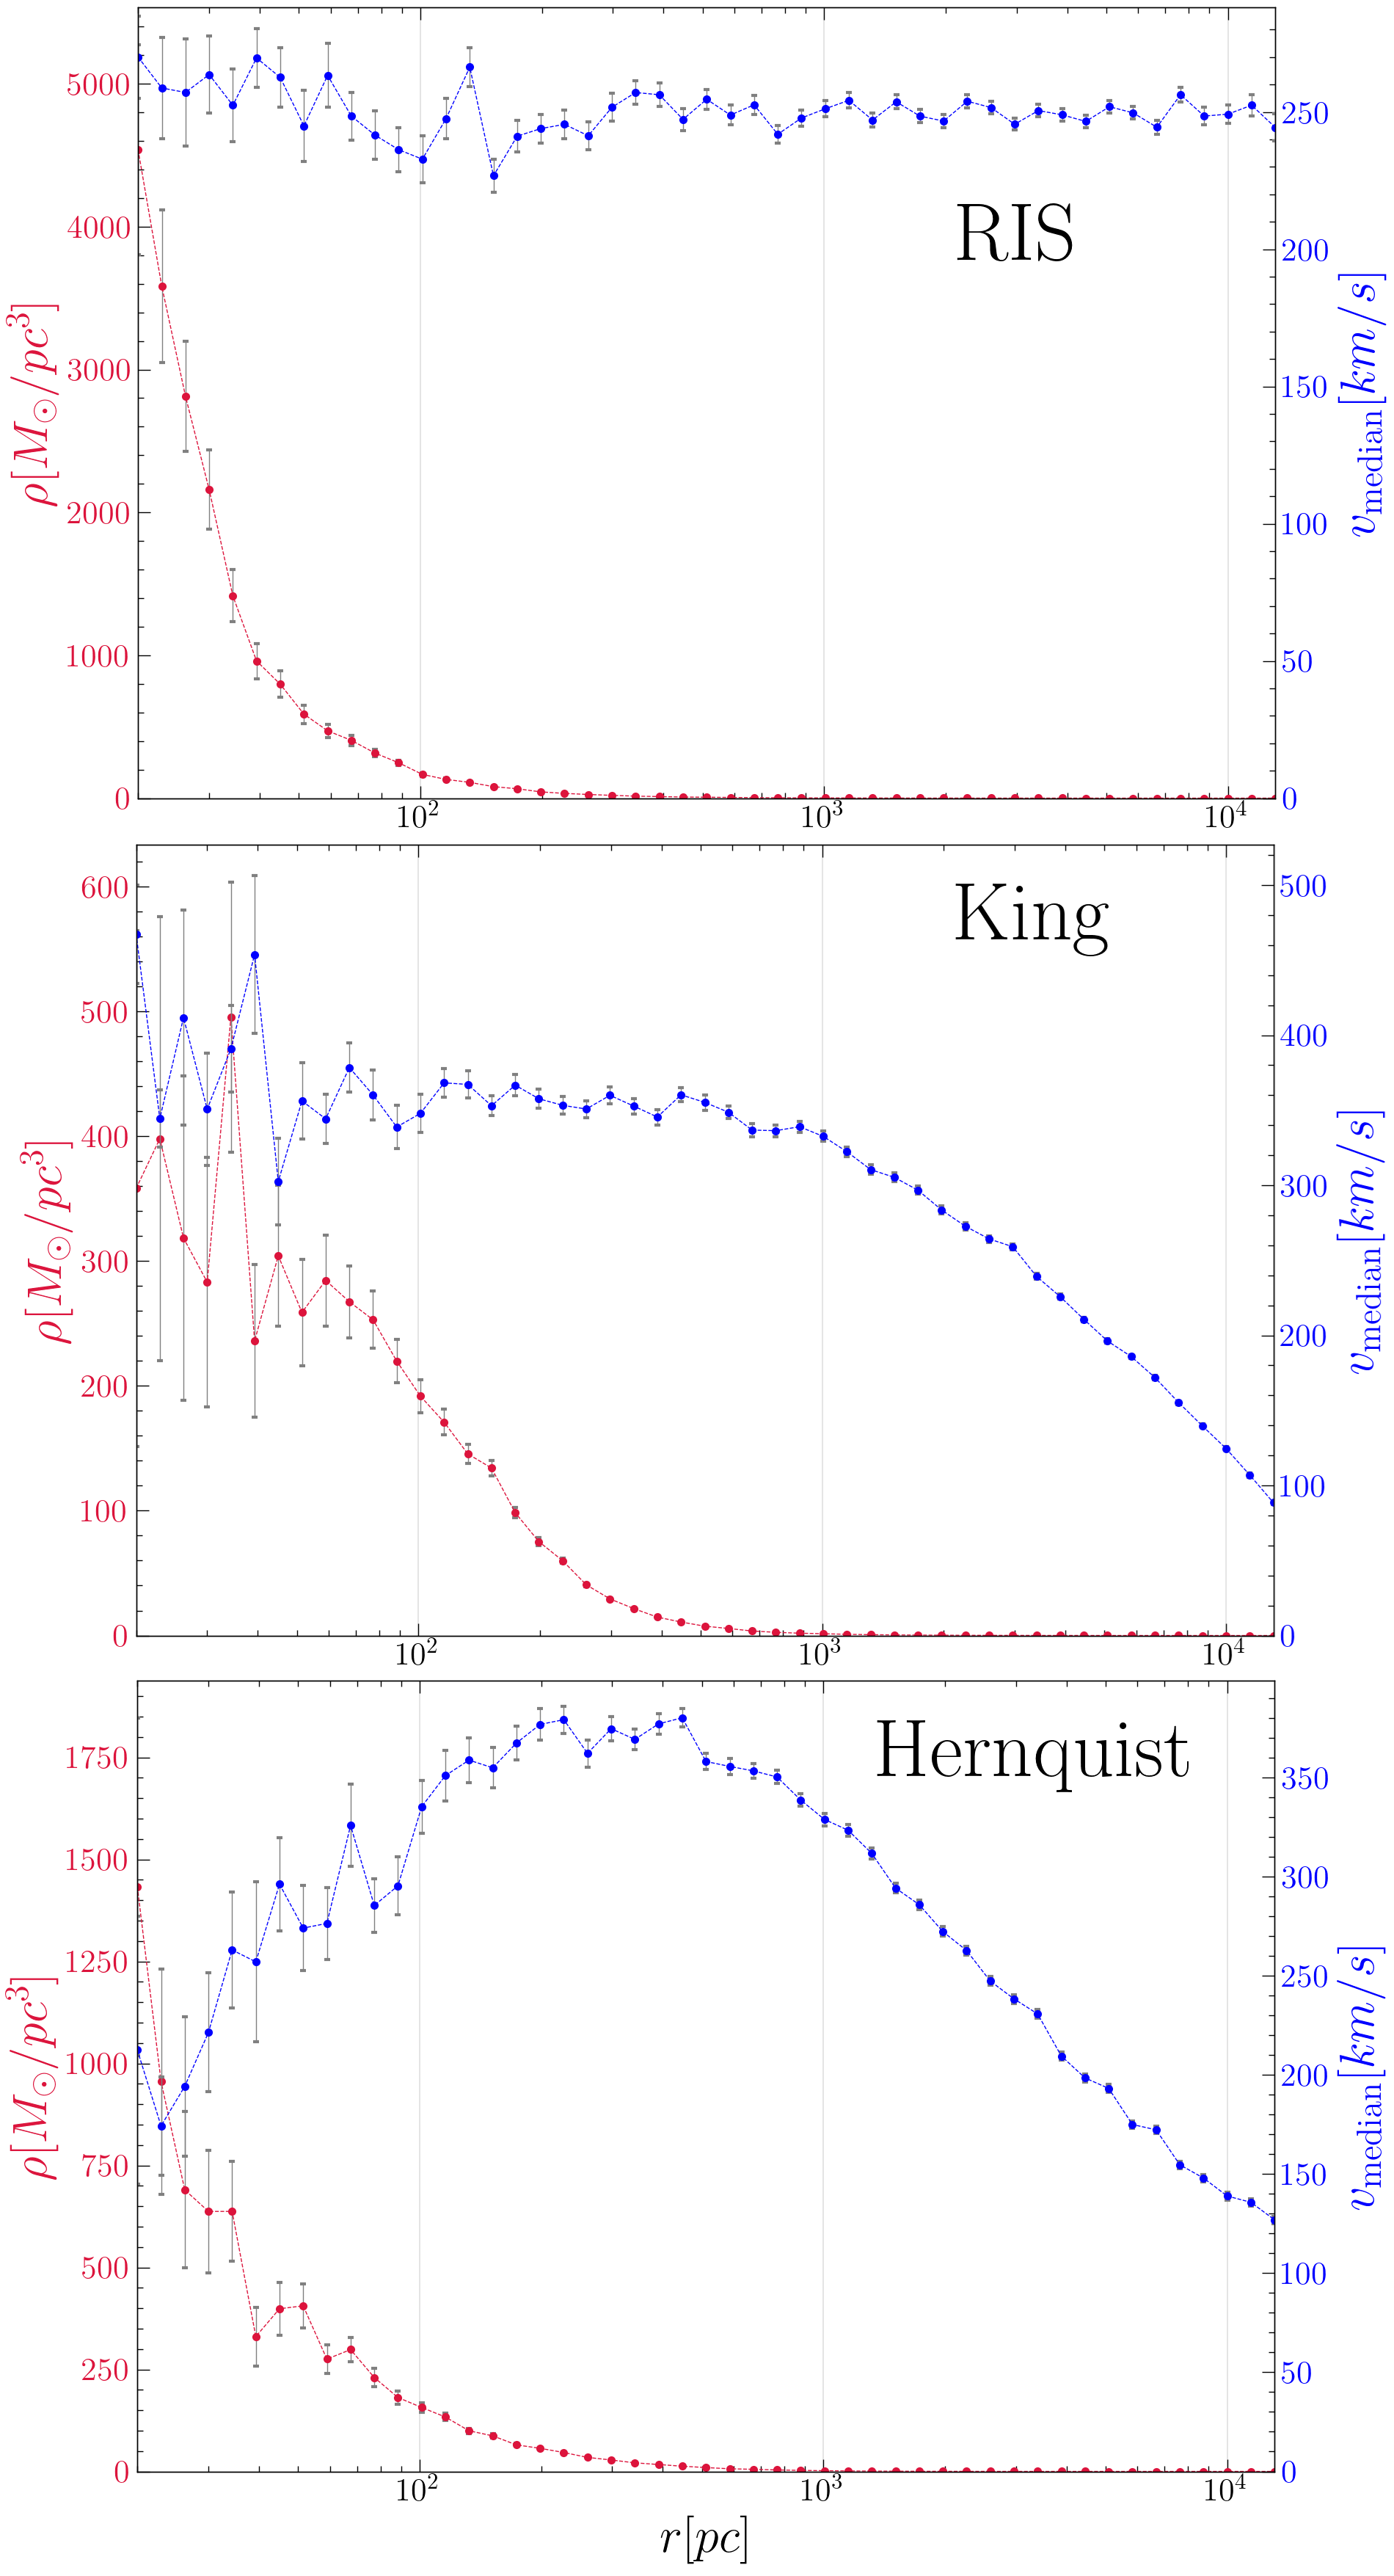
\includegraphics[width=1.\columnwidth]{Profiles.png}
    \caption{Mass density (red) and median velocity (blue) as a function of the distance from the center of mass at the initial time $t=0$ for the RIS model (upper panel), the King model (middle panel), and the Hernquist model (lower panel). The errors on the density have been computed by assuming Poissonian fluctuations in the number of particles within each spherical shell, while the errors on the velocity are proportional to the interquartile range.}
    \label{fig:profiles}
\end{figure}

\begin{figure}\centering
	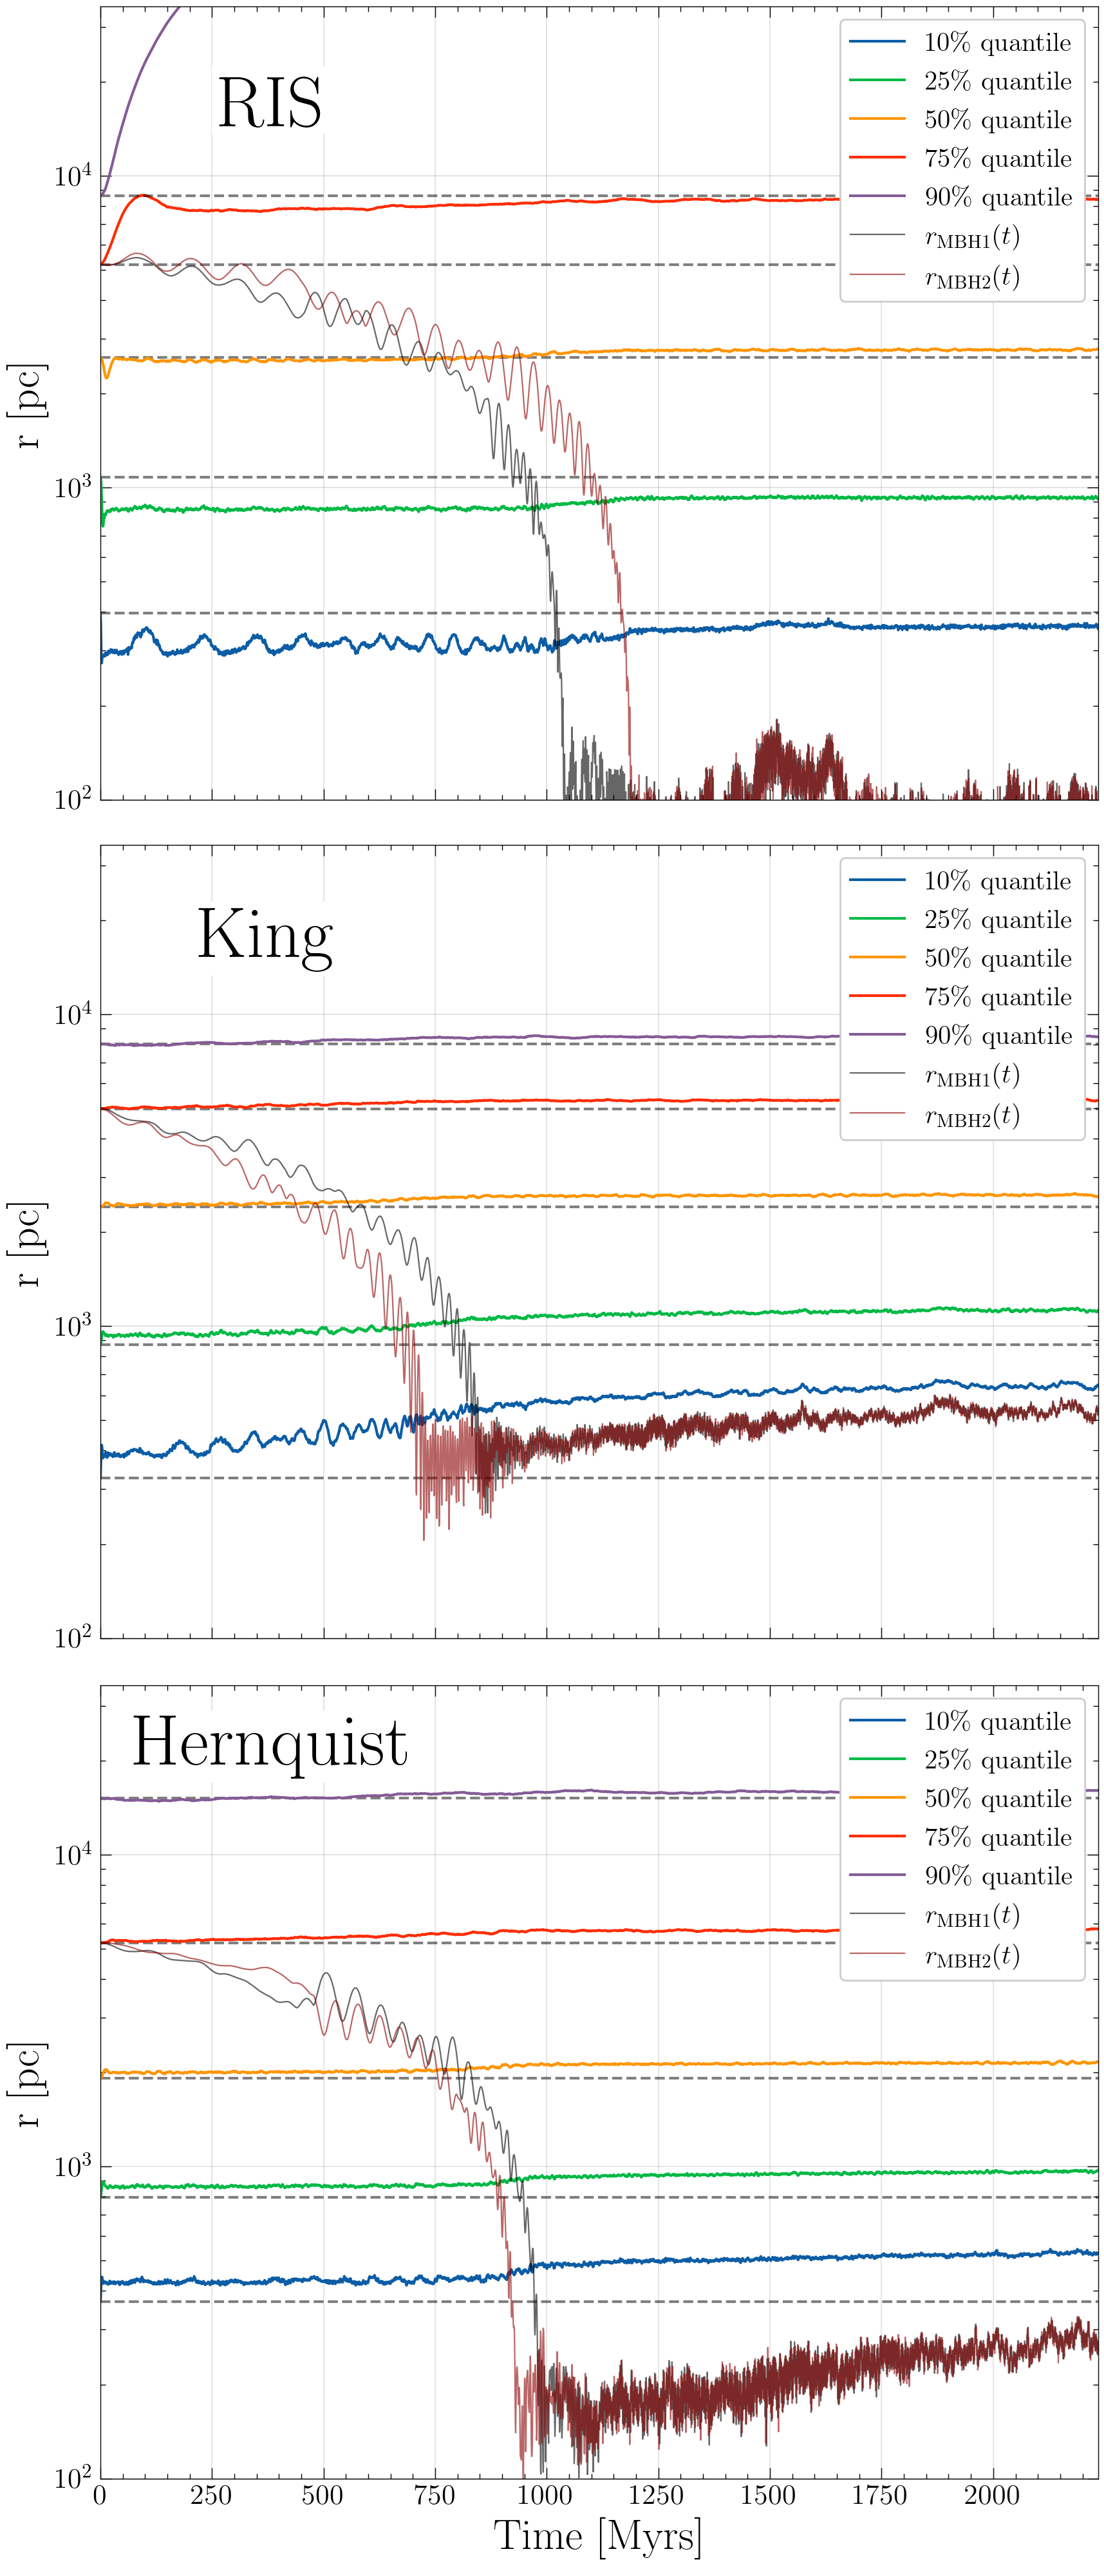
\includegraphics[width=0.9\columnwidth]{LR_50K_dt0005_titles.png}
    \caption{Time evolution of the Lagrangian radii for the RIS model (upper panel), the King model (middle panel), and the Hernquist model (lower panel). The trajectories of the two SMBHs are shown in black and red.}
    \label{fig:Lagrangian_radii}
\end{figure}

\begin{figure}\centering
	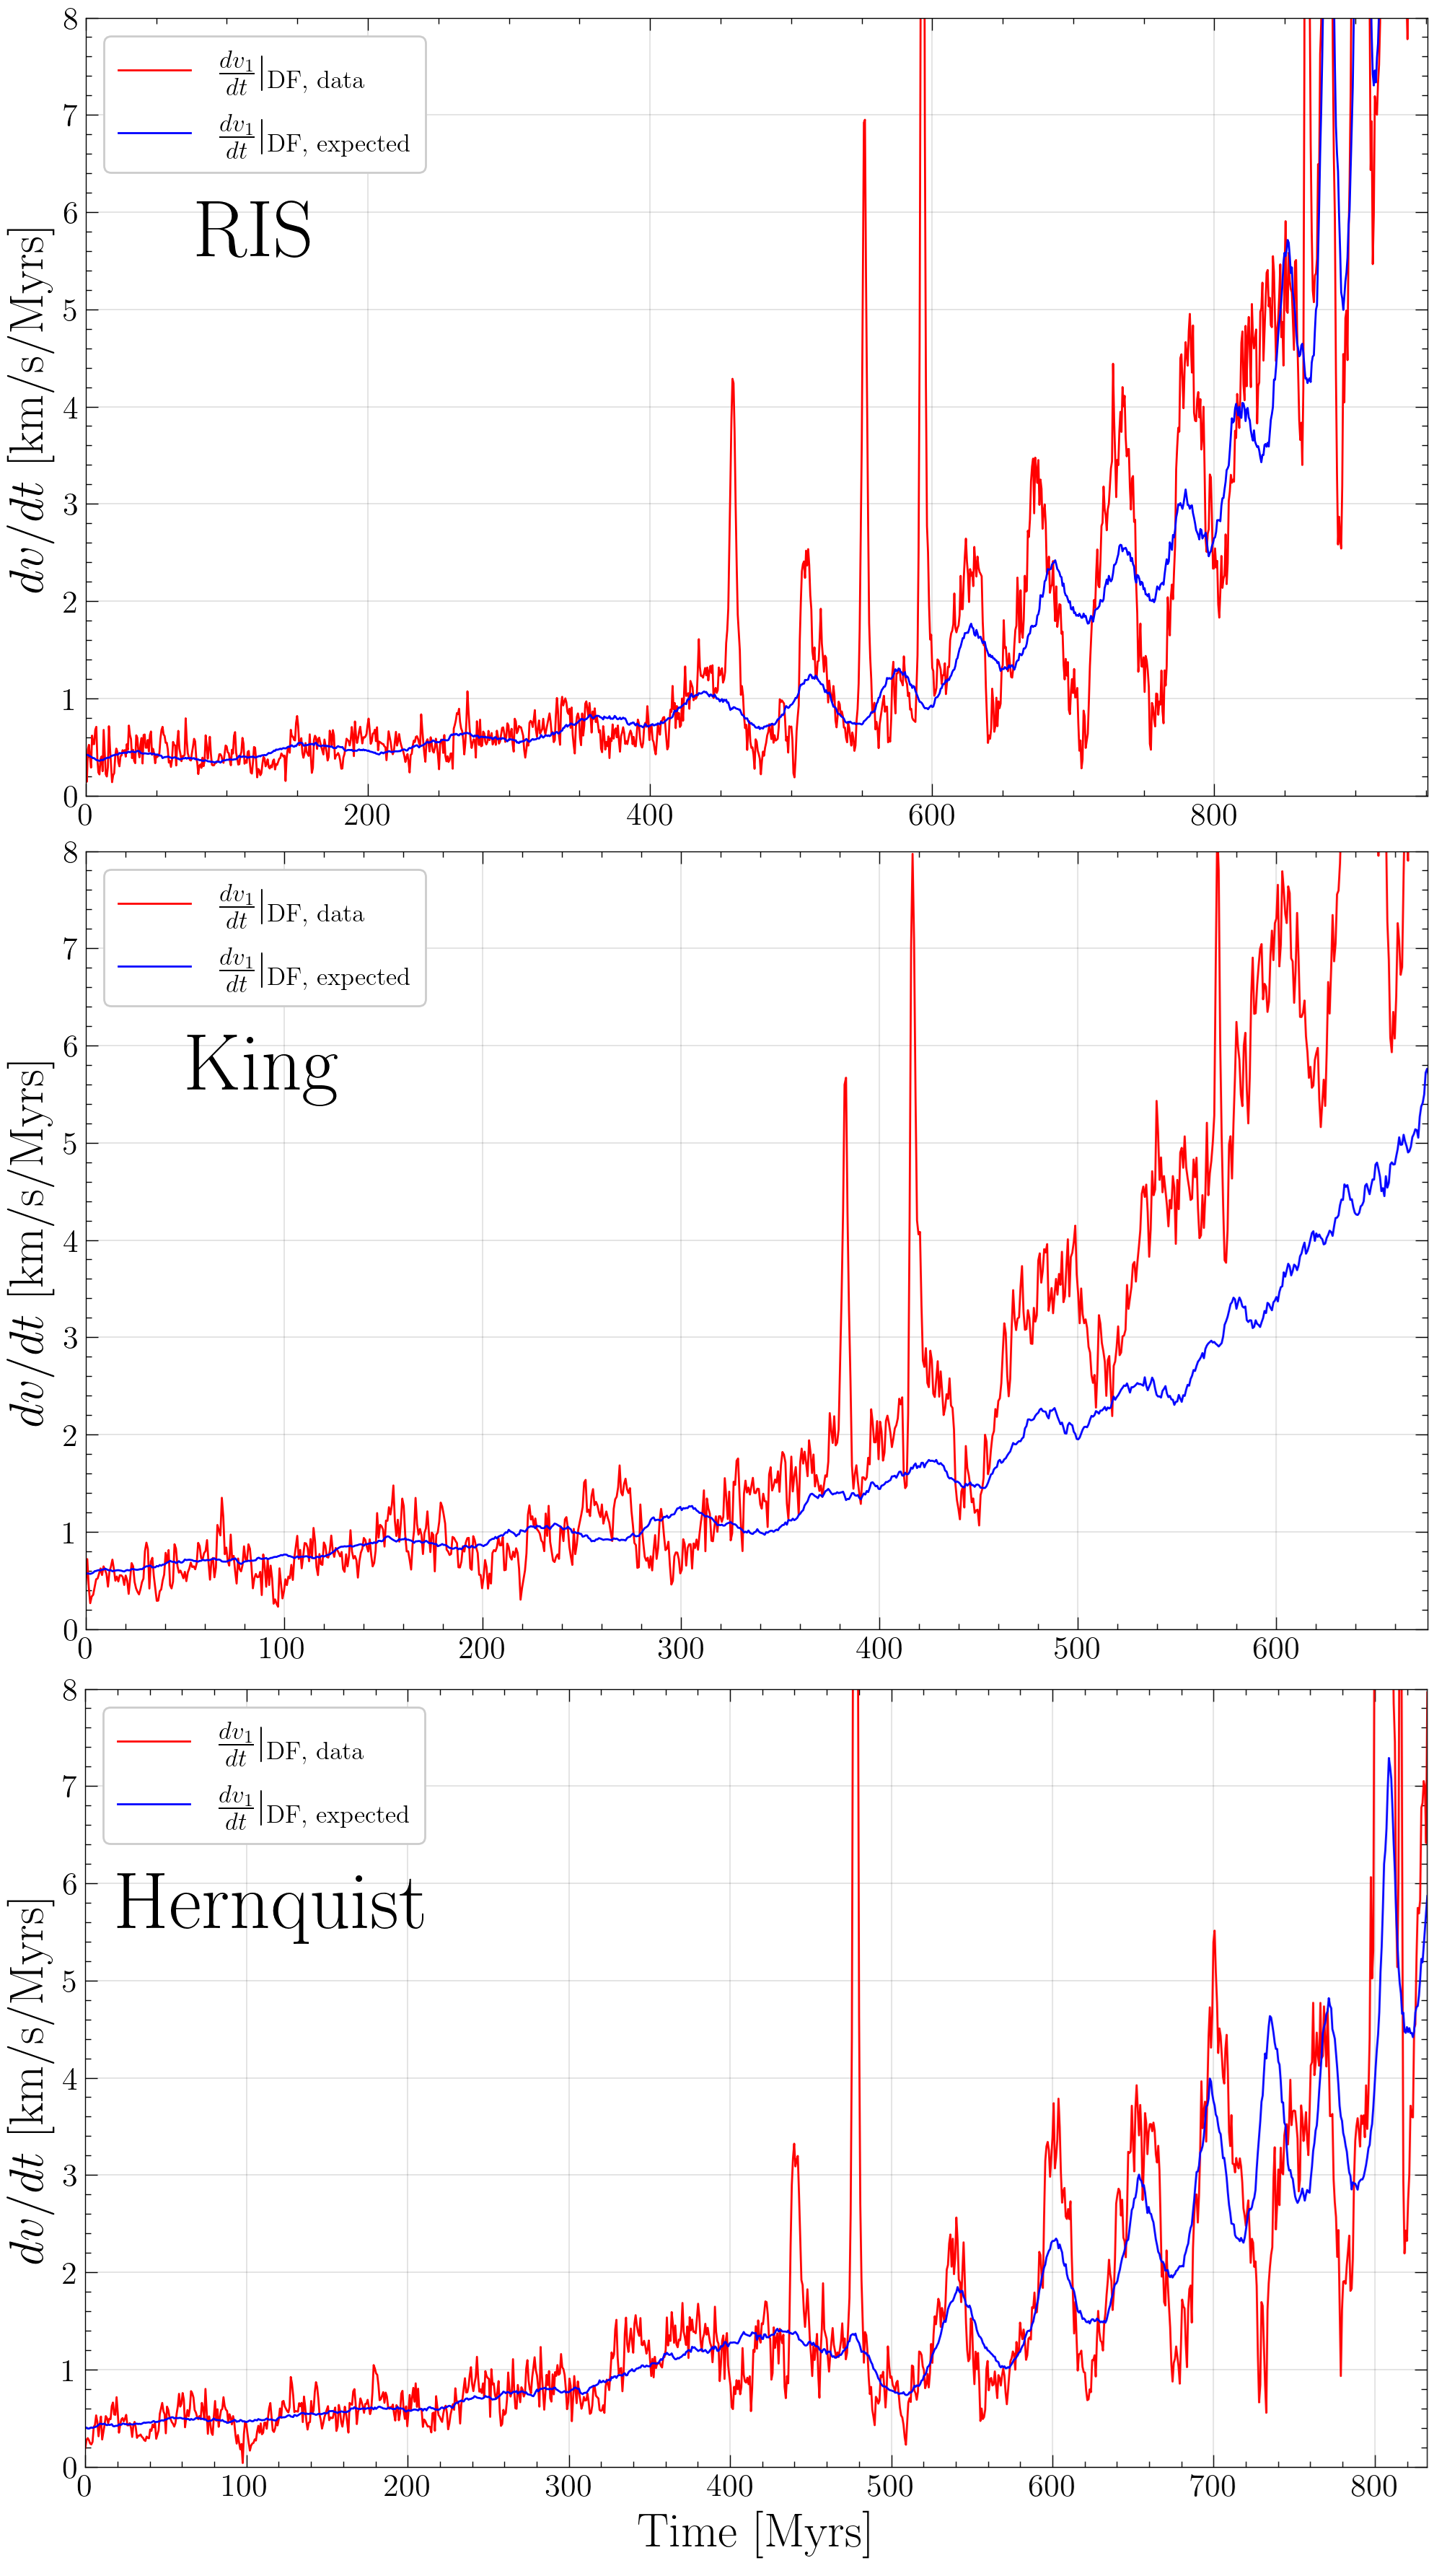
\includegraphics[width=1.\columnwidth]{Acceleration.png}
    \caption{Comparison between the net acceleration of one SMBH (red) and the theoretical dynamical friction acceleration (blue) as a function of time for the RIS model (upper panel), the King model (middle panel), and the Hernquist model (lower panel).}
    \label{fig:Acceleration}
\end{figure}

\begin{figure}\centering
	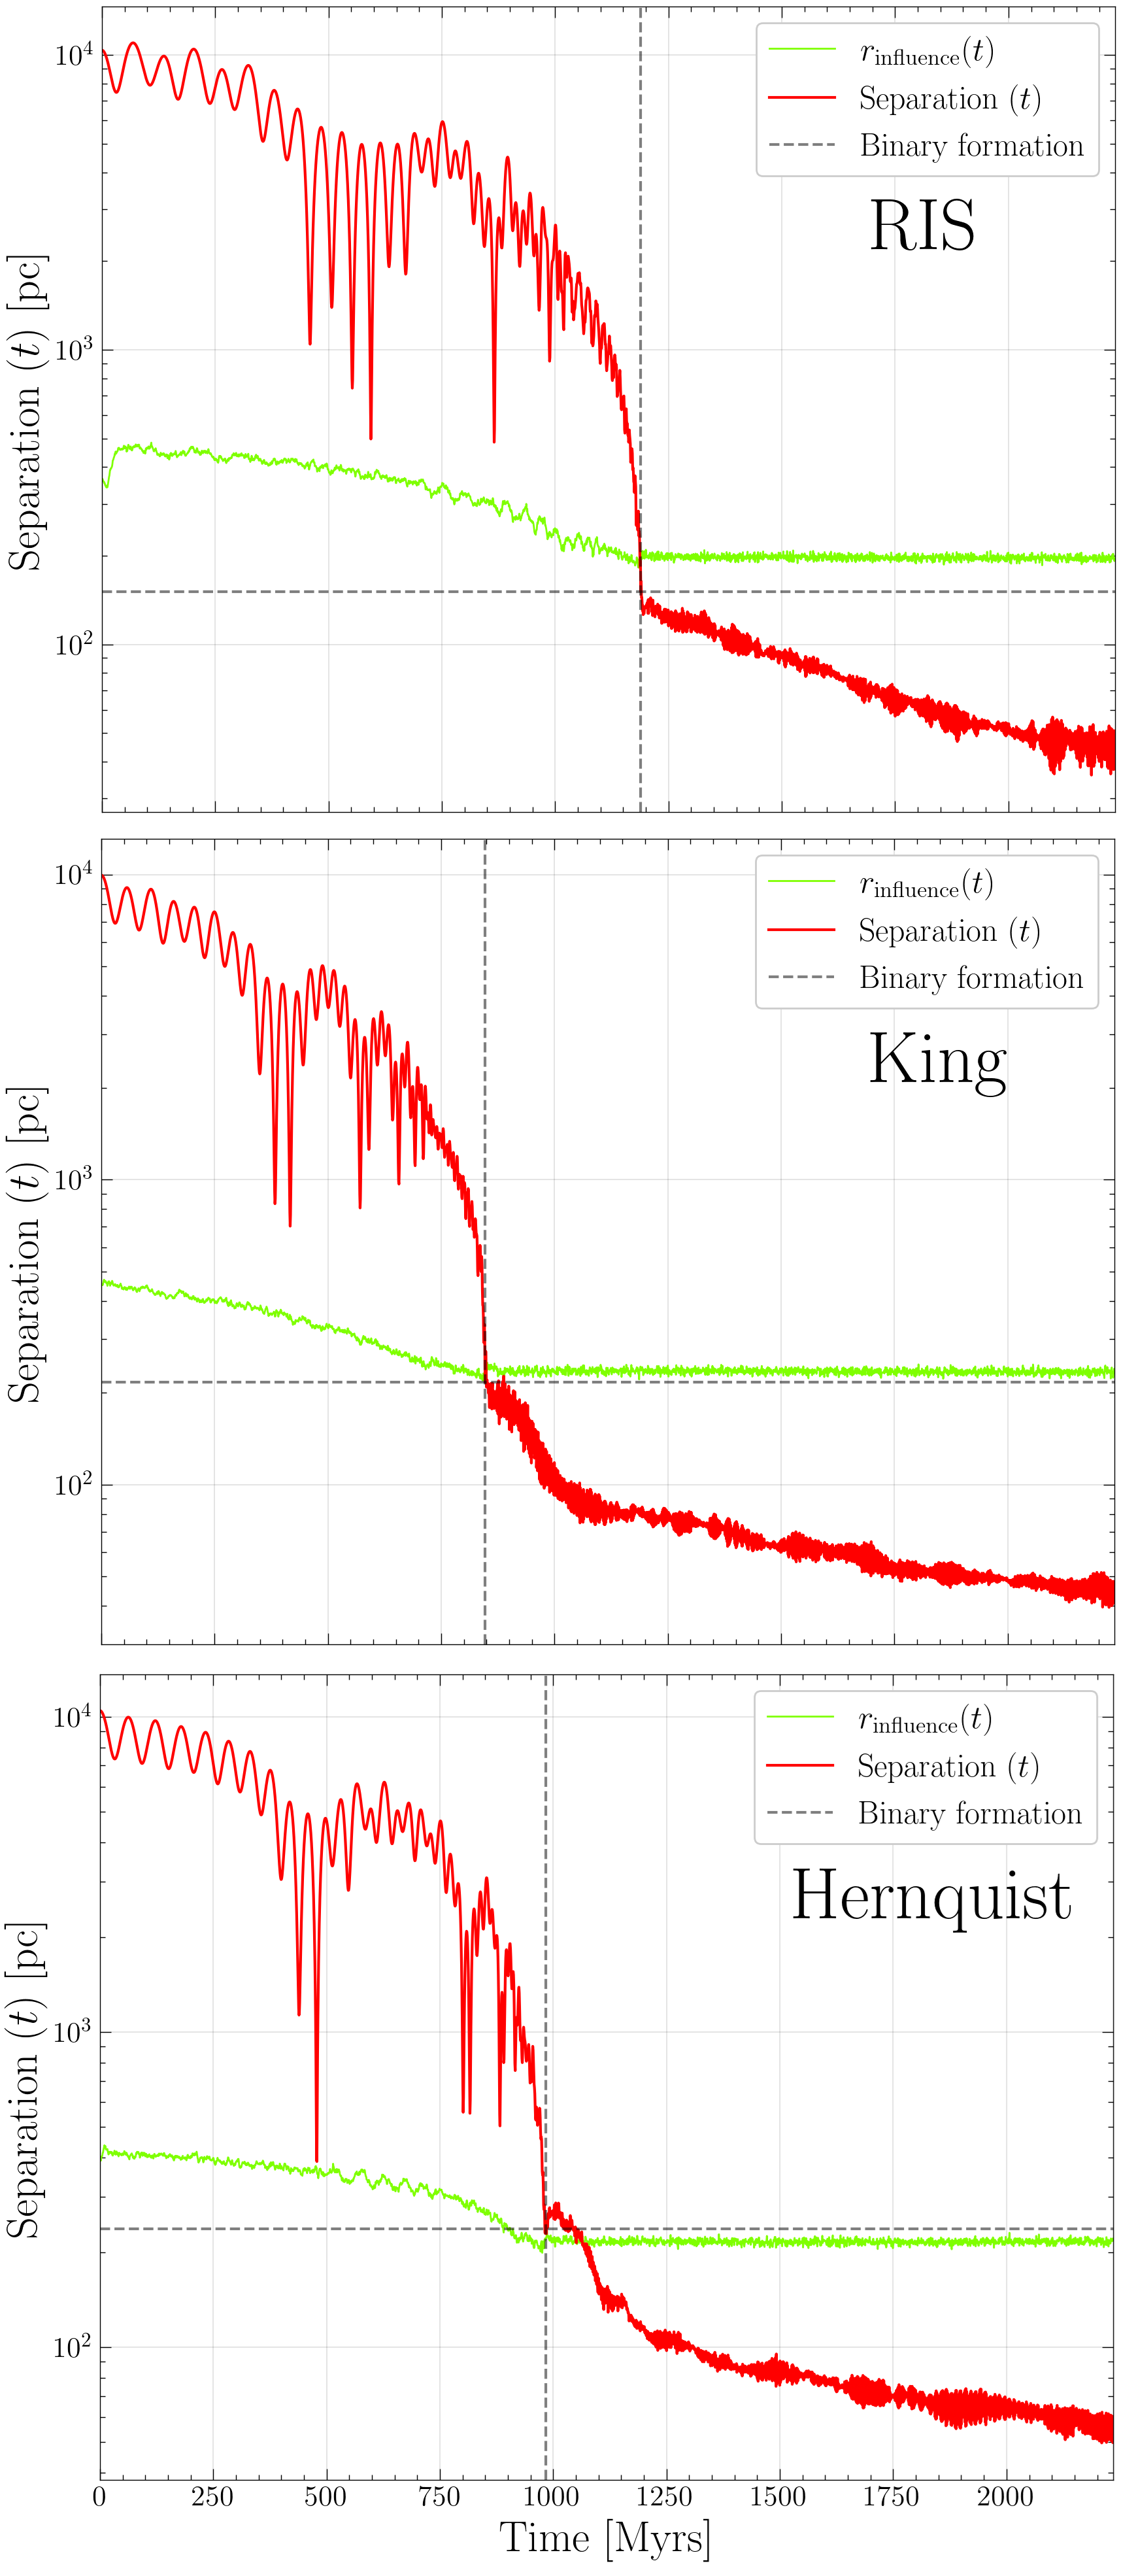
\includegraphics[width=0.9\columnwidth]{Separation.png}
    \caption{Time evolution of the SMBHs separation (red) for the RIS model (upper panel), the King model (middle panel), and the Hernquist model (lower panel). The mean influence radius (green) is also shown. The dashed lines indicate the time and the separation at which the binary forms.}
    \label{fig:Separation}
\end{figure}

%%%%%%%%%%%%%%%%%%%% REFERENCES %%%%%%%%%%%%%%%%%%%%%%%%%%%%%%%%%%%%%%%%%%%%%%%%%%%%%%%%%%%%%%%%%%%%
% The best way to enter references is to use BibTeX:
\nocite{*}
\bibliographystyle{mnras}
\bibliography{bibliography} 
%%%%%%%%%%%%%%%%%%%%%%%%%%%%%%%%%%%%%%%%%%%%%%%%%%%%%%%%%%%%%%%%%%%%%%%%%%%%%%%%%%%%%%%%%%%%%%%%%%%%


% Don't change these lines
\label{lastpage}
\end{document}
